% Options for packages loaded elsewhere
\PassOptionsToPackage{unicode}{hyperref}
\PassOptionsToPackage{hyphens}{url}
\PassOptionsToPackage{dvipsnames,svgnames,x11names}{xcolor}
%
\documentclass[
  11pt,
  a4paper,
  DIV=11,
  numbers=noendperiod]{scrartcl}

\usepackage{amsmath,amssymb}
\usepackage{iftex}
\ifPDFTeX
  \usepackage[T1]{fontenc}
  \usepackage[utf8]{inputenc}
  \usepackage{textcomp} % provide euro and other symbols
\else % if luatex or xetex
  \usepackage{unicode-math}
  \defaultfontfeatures{Scale=MatchLowercase}
  \defaultfontfeatures[\rmfamily]{Ligatures=TeX,Scale=1}
\fi
\usepackage{lmodern}
\ifPDFTeX\else  
    % xetex/luatex font selection
    \setmainfont[]{Avenir Next}
\fi
% Use upquote if available, for straight quotes in verbatim environments
\IfFileExists{upquote.sty}{\usepackage{upquote}}{}
\IfFileExists{microtype.sty}{% use microtype if available
  \usepackage[]{microtype}
  \UseMicrotypeSet[protrusion]{basicmath} % disable protrusion for tt fonts
}{}
\makeatletter
\@ifundefined{KOMAClassName}{% if non-KOMA class
  \IfFileExists{parskip.sty}{%
    \usepackage{parskip}
  }{% else
    \setlength{\parindent}{0pt}
    \setlength{\parskip}{6pt plus 2pt minus 1pt}}
}{% if KOMA class
  \KOMAoptions{parskip=half}}
\makeatother
\usepackage{xcolor}
\usepackage[top=3cm, bottom=2cm, left=4cm, right=2cm]{geometry}
\setlength{\emergencystretch}{3em} % prevent overfull lines
\setcounter{secnumdepth}{-\maxdimen} % remove section numbering
% Make \paragraph and \subparagraph free-standing
\makeatletter
\ifx\paragraph\undefined\else
  \let\oldparagraph\paragraph
  \renewcommand{\paragraph}{
    \@ifstar
      \xxxParagraphStar
      \xxxParagraphNoStar
  }
  \newcommand{\xxxParagraphStar}[1]{\oldparagraph*{#1}\mbox{}}
  \newcommand{\xxxParagraphNoStar}[1]{\oldparagraph{#1}\mbox{}}
\fi
\ifx\subparagraph\undefined\else
  \let\oldsubparagraph\subparagraph
  \renewcommand{\subparagraph}{
    \@ifstar
      \xxxSubParagraphStar
      \xxxSubParagraphNoStar
  }
  \newcommand{\xxxSubParagraphStar}[1]{\oldsubparagraph*{#1}\mbox{}}
  \newcommand{\xxxSubParagraphNoStar}[1]{\oldsubparagraph{#1}\mbox{}}
\fi
\makeatother

\usepackage{color}
\usepackage{fancyvrb}
\newcommand{\VerbBar}{|}
\newcommand{\VERB}{\Verb[commandchars=\\\{\}]}
\DefineVerbatimEnvironment{Highlighting}{Verbatim}{commandchars=\\\{\}}
% Add ',fontsize=\small' for more characters per line
\usepackage{framed}
\definecolor{shadecolor}{RGB}{241,243,245}
\newenvironment{Shaded}{\begin{snugshade}}{\end{snugshade}}
\newcommand{\AlertTok}[1]{\textcolor[rgb]{0.68,0.00,0.00}{#1}}
\newcommand{\AnnotationTok}[1]{\textcolor[rgb]{0.37,0.37,0.37}{#1}}
\newcommand{\AttributeTok}[1]{\textcolor[rgb]{0.40,0.45,0.13}{#1}}
\newcommand{\BaseNTok}[1]{\textcolor[rgb]{0.68,0.00,0.00}{#1}}
\newcommand{\BuiltInTok}[1]{\textcolor[rgb]{0.00,0.23,0.31}{#1}}
\newcommand{\CharTok}[1]{\textcolor[rgb]{0.13,0.47,0.30}{#1}}
\newcommand{\CommentTok}[1]{\textcolor[rgb]{0.37,0.37,0.37}{#1}}
\newcommand{\CommentVarTok}[1]{\textcolor[rgb]{0.37,0.37,0.37}{\textit{#1}}}
\newcommand{\ConstantTok}[1]{\textcolor[rgb]{0.56,0.35,0.01}{#1}}
\newcommand{\ControlFlowTok}[1]{\textcolor[rgb]{0.00,0.23,0.31}{\textbf{#1}}}
\newcommand{\DataTypeTok}[1]{\textcolor[rgb]{0.68,0.00,0.00}{#1}}
\newcommand{\DecValTok}[1]{\textcolor[rgb]{0.68,0.00,0.00}{#1}}
\newcommand{\DocumentationTok}[1]{\textcolor[rgb]{0.37,0.37,0.37}{\textit{#1}}}
\newcommand{\ErrorTok}[1]{\textcolor[rgb]{0.68,0.00,0.00}{#1}}
\newcommand{\ExtensionTok}[1]{\textcolor[rgb]{0.00,0.23,0.31}{#1}}
\newcommand{\FloatTok}[1]{\textcolor[rgb]{0.68,0.00,0.00}{#1}}
\newcommand{\FunctionTok}[1]{\textcolor[rgb]{0.28,0.35,0.67}{#1}}
\newcommand{\ImportTok}[1]{\textcolor[rgb]{0.00,0.46,0.62}{#1}}
\newcommand{\InformationTok}[1]{\textcolor[rgb]{0.37,0.37,0.37}{#1}}
\newcommand{\KeywordTok}[1]{\textcolor[rgb]{0.00,0.23,0.31}{\textbf{#1}}}
\newcommand{\NormalTok}[1]{\textcolor[rgb]{0.00,0.23,0.31}{#1}}
\newcommand{\OperatorTok}[1]{\textcolor[rgb]{0.37,0.37,0.37}{#1}}
\newcommand{\OtherTok}[1]{\textcolor[rgb]{0.00,0.23,0.31}{#1}}
\newcommand{\PreprocessorTok}[1]{\textcolor[rgb]{0.68,0.00,0.00}{#1}}
\newcommand{\RegionMarkerTok}[1]{\textcolor[rgb]{0.00,0.23,0.31}{#1}}
\newcommand{\SpecialCharTok}[1]{\textcolor[rgb]{0.37,0.37,0.37}{#1}}
\newcommand{\SpecialStringTok}[1]{\textcolor[rgb]{0.13,0.47,0.30}{#1}}
\newcommand{\StringTok}[1]{\textcolor[rgb]{0.13,0.47,0.30}{#1}}
\newcommand{\VariableTok}[1]{\textcolor[rgb]{0.07,0.07,0.07}{#1}}
\newcommand{\VerbatimStringTok}[1]{\textcolor[rgb]{0.13,0.47,0.30}{#1}}
\newcommand{\WarningTok}[1]{\textcolor[rgb]{0.37,0.37,0.37}{\textit{#1}}}

\providecommand{\tightlist}{%
  \setlength{\itemsep}{0pt}\setlength{\parskip}{0pt}}\usepackage{longtable,booktabs,array}
\usepackage{calc} % for calculating minipage widths
% Correct order of tables after \paragraph or \subparagraph
\usepackage{etoolbox}
\makeatletter
\patchcmd\longtable{\par}{\if@noskipsec\mbox{}\fi\par}{}{}
\makeatother
% Allow footnotes in longtable head/foot
\IfFileExists{footnotehyper.sty}{\usepackage{footnotehyper}}{\usepackage{footnote}}
\makesavenoteenv{longtable}
\usepackage{graphicx}
\makeatletter
\newsavebox\pandoc@box
\newcommand*\pandocbounded[1]{% scales image to fit in text height/width
  \sbox\pandoc@box{#1}%
  \Gscale@div\@tempa{\textheight}{\dimexpr\ht\pandoc@box+\dp\pandoc@box\relax}%
  \Gscale@div\@tempb{\linewidth}{\wd\pandoc@box}%
  \ifdim\@tempb\p@<\@tempa\p@\let\@tempa\@tempb\fi% select the smaller of both
  \ifdim\@tempa\p@<\p@\scalebox{\@tempa}{\usebox\pandoc@box}%
  \else\usebox{\pandoc@box}%
  \fi%
}
% Set default figure placement to htbp
\def\fps@figure{htbp}
\makeatother

\usepackage[document]{ragged2e}
\KOMAoption{captions}{tableheading}
\makeatletter
\@ifpackageloaded{caption}{}{\usepackage{caption}}
\AtBeginDocument{%
\ifdefined\contentsname
  \renewcommand*\contentsname{Table of contents}
\else
  \newcommand\contentsname{Table of contents}
\fi
\ifdefined\listfigurename
  \renewcommand*\listfigurename{List of Figures}
\else
  \newcommand\listfigurename{List of Figures}
\fi
\ifdefined\listtablename
  \renewcommand*\listtablename{List of Tables}
\else
  \newcommand\listtablename{List of Tables}
\fi
\ifdefined\figurename
  \renewcommand*\figurename{Figure}
\else
  \newcommand\figurename{Figure}
\fi
\ifdefined\tablename
  \renewcommand*\tablename{Table}
\else
  \newcommand\tablename{Table}
\fi
}
\@ifpackageloaded{float}{}{\usepackage{float}}
\floatstyle{ruled}
\@ifundefined{c@chapter}{\newfloat{codelisting}{h}{lop}}{\newfloat{codelisting}{h}{lop}[chapter]}
\floatname{codelisting}{Listing}
\newcommand*\listoflistings{\listof{codelisting}{List of Listings}}
\makeatother
\makeatletter
\makeatother
\makeatletter
\@ifpackageloaded{caption}{}{\usepackage{caption}}
\@ifpackageloaded{subcaption}{}{\usepackage{subcaption}}
\makeatother

\usepackage{bookmark}

\IfFileExists{xurl.sty}{\usepackage{xurl}}{} % add URL line breaks if available
\urlstyle{same} % disable monospaced font for URLs
\hypersetup{
  pdftitle={2. Hello World Python},
  colorlinks=true,
  linkcolor={blue},
  filecolor={Maroon},
  citecolor={Blue},
  urlcolor={Blue},
  pdfcreator={LaTeX via pandoc}}


\title{2. Hello World Python}
\author{}
\date{}

\begin{document}
\maketitle


\subsection{2.1 Kurze Geschichte der
Programmiersprachen}\label{kurze-geschichte-der-programmiersprachen}

\begin{enumerate}
\def\labelenumi{\arabic{enumi}.}
\item
  Generation: Programmierung im Maschinencode.
\item
  Generation: Assemblersprachen und erste Entwicklung höherer
  Programmiersprachen wie FORTRAN, ALGOL und COBOL.
\item
  Generation: Entwicklung von Betriebssytemen mit Dialogbetrieb,
  Datenbanken, Methoden der strukturierten Programmierung,
  Programmiersprache Pascal
\item
  Generation: verteilte Systeme, Rechnernetze, Kommunikationsfähigkeit,
  gute Arbeits- und Programmierumgebungen;
\item
  Generation: Wissensverarbeitung, automatisches Schlussfolgern,
  deduktive Datenbanken, Expertensysteme, PROLOG.
\end{enumerate}

Heute gibt es eine unübersehbare Fülle von Programmiersprachen, für die
verschiedensten Anwendungsgebiete. Nur wenige Programmiersprachen haben
jedoch als universell verwendbare Sprachen einen hohen Verbreitungsgrad
in der industriellen Praxis erreicht.

Programmiersprachen werden üblicherweise Sprachen in folgende vier
großen Klassen zu unterteilen:

\begin{enumerate}
\def\labelenumi{\arabic{enumi}.}
\item
  Imperative Sprachen: Beispiele sind Basic, Algol, Pascal, FORTRAN, C,
  Modula
\item
  Funktionale Sprachen: Beispiele sind LISP, ML, Haskell
\item
  Logische Sprachen: Hier ist PROLOG das bekannteste Beispiel
\item
  Objektorientierte Sprachen: Smalltalk, Simula, C++ und Java gehören in
  diese Klasse.
\end{enumerate}

Und Python? Dazu später.

Die Zuordnung einer Sprache zu einer dieser Klassen ist nicht immer
eindeutig möglich. So haben beispielsweise die objektorientierten
Sprachen C++ und Java einen imperativen Sprachkern und könnten so ebenso
der Klasse der imperativen Sprachen zugeordnet werden. Die vier
Sprachklassen kennzeichnen daher eher einen gewissen Programmier-Stil
und weniger die Ausdrucksfähigkeit einer bestimmten Sprache.

\subsection{2.2 Kurze Geschiche von
Python}\label{kurze-geschiche-von-python}

\begin{itemize}
\tightlist
\item
  Python wurde von dem niederländischen Informatiker Guido van Rossum
  entwickelt
\item
  Die Entwicklung begann Ende der 1980er Jahre als Hobbyprojekt
\end{itemize}


\includegraphics[width=2.60417in,height=\textheight,keepaspectratio]{images/nosnake.jpg}

\includegraphics[width=2.60417in,height=\textheight,keepaspectratio]{images/montypython.jpg}

\begin{itemize}
\item
  Der Name sollte kurz, einprägsam und etwas unkonventionell sein, um
  die Philosophie von Python widerzuspiegeln. van Rossum war ein großer
  Fan der britischen Comedy-Show ``Monty Python's Flying Circus'', daher
  der Name ``Python''.
\item
  Meilensteine:

  \begin{itemize}
  \tightlist
  \item
    \textbf{Python 0.9.0 (1991)} Die erste Version, Python 0.9.0, wurde
    im Februar 1991 veröffentlicht.
  \item
    \textbf{Python 1.0 (1994):} Die erste offizielle Version von Python
    wurde veröffentlicht und legte den Grundstein für die weitere
    Entwicklung der Sprache.
  \item
    \textbf{Python 2.0 (2000):} List Comprehensions wurden eingeführt,
    um das Erstellen von Listen auf eine elegante und kompakte Weise zu
    ermöglichen.
  \item
    \textbf{Gründung der Python Software Foundation (PSF) (2001):} Die
    PSF wurde gegründet, um die Weiterentwicklung und Verbreitung von
    Python zu unterstützen. Sie spielt eine wichtige Rolle in der
    Förderung und Verwaltung der Python-Community.
  \item
    \textbf{Python 3.x (2008):} Python 3.0 wurde veröffentlicht und
    führte tiefgreifende Veränderungen in der Sprache ein, um einige
    Probleme und Unklarheiten in Python 2.x zu beheben. Diese Versionen
    existierten eine Zeit lang nebeneinander, was zu Diskussionen in der
    Community führte.
  \end{itemize}
\end{itemize}

\subsection{2.3 Eigenschaften von
Python}\label{eigenschaften-von-python}

\textbf{Allgemein}

\begin{itemize}
\tightlist
\item
  einfach erlernbar und lesbar
\item
  Interpreter-basiert
\item
  plattformunabhängig
\item
  Open Source
\end{itemize}

\textbf{Sprachparadigmen:} - imperativ: Ein Programm besteht aus einer
Folge von Anweisungen (Befehlen), die den Zustand des Programms Schritt
für Schritt verändern. - prozedural: Ein Programm wird in Prozeduren
(auch Funktionen oder Routinen genannt) unterteiltS. Sie ist eine
Unterform der imperativen Programmierung. Dabei wird der Code in
wiederverwendbare, logisch zusammengehörige Blöcke aufgeteilt, die
bestimmte Aufgaben übernehmen. - objektorientiert: Python unterstützt
Klassen, Objekte, Vererbung usw. - funktional: Ein Programme kann durch
das Anwenden und Kombinieren von Funktionen aufgebaut werden. Python ist
aber nicht rein funktional. - dynamisch typisiert: Keine
Typdeklarationen notwendig. Der Typ eines Variablen wird beim
Verarbeiten des Programms bestimmt.

\(\Rightarrow\) Python ist eine Mehrparadigmen-Programmiersprache, die
verschiedene Programmieransätze unterstützt.

\subsection{2.4 Der Python-Interpreter}\label{der-python-interpreter}

\textbf{Compilierte Sprachen vs interpretierte Sprache}

Python ist eine interpretierte Programmiersprache. Im Gegensatz zu
compilierten Sprachen, bei denen der Quellcode vom Compiler in
Maschinencode übersetzt wird, der direkt vom Prozessor ausgeführt werden
kann, wird bei Python com Compiler ein sogenannter Bytecode erzeugt.
Dieser Bytecode wird anschließend vom Python-Interpreter zeilenweise
ausgeführt. Das ermöglicht eine schnelle Entwicklung, einfaches
Debugging und hohe Flexibilität während des Programmierens. Insbesondere
kann man auf diese Weise plattformunabhängig programmieren, da der
Python-Interpreter (PVM = Python-Virtual-Machine) auf verschiedenen
Betriebssystemen verfügbar ist.

Ablauf compilierte Sprachen vs interpretierte Sprachen:

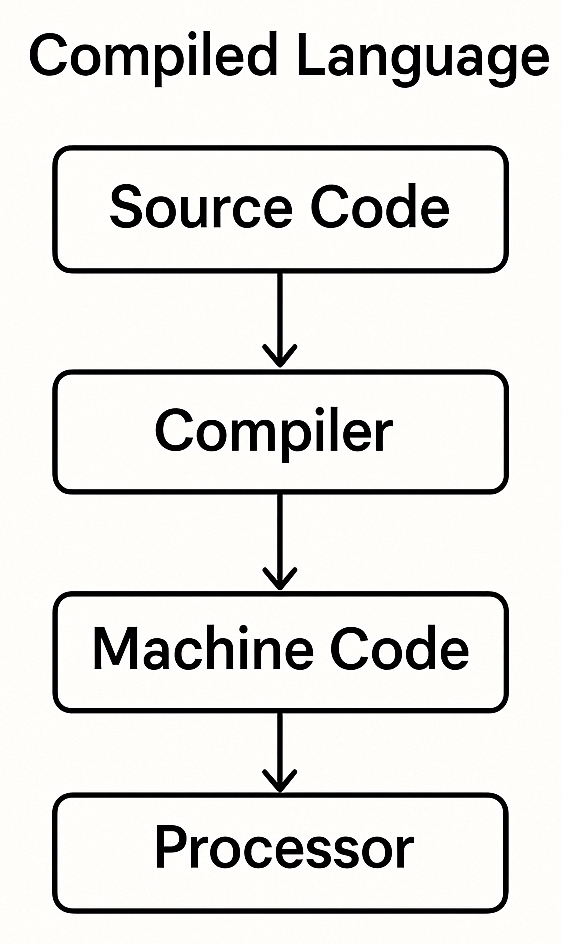
\includegraphics[width=1.5625in,height=\textheight,keepaspectratio]{images/compiler.jpg}
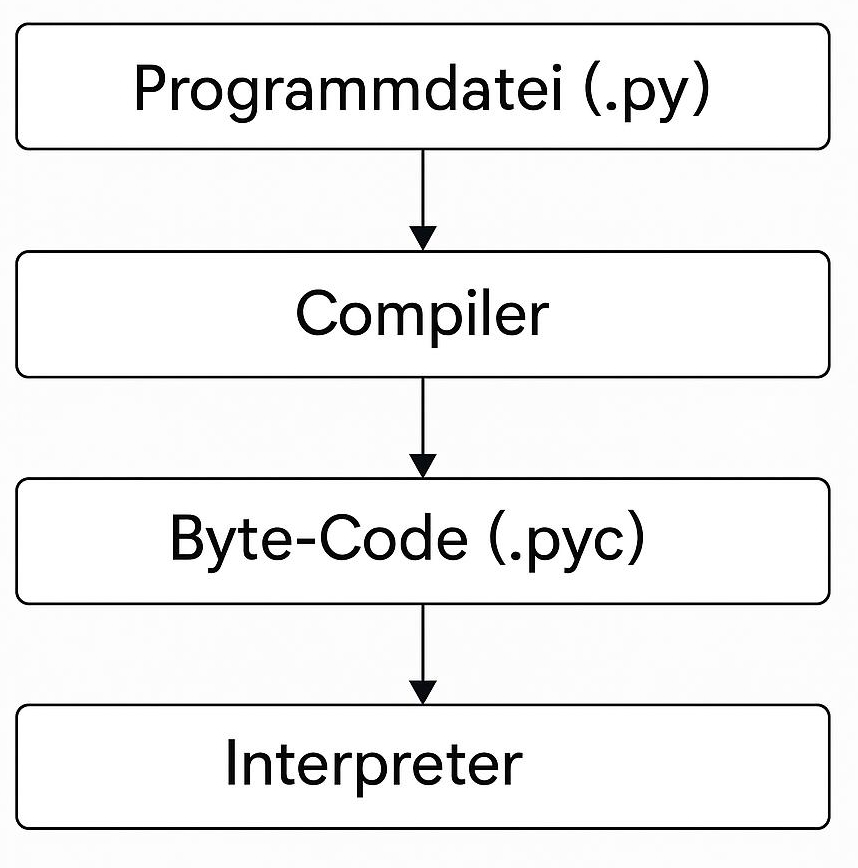
\includegraphics[width=2.29167in,height=\textheight,keepaspectratio]{images/interpreter.jpg}

\textbf{direkte Kommunikation mit dem Python Interpreter}

Die direkte Kommunikation mit Python bezeichnet die unmittelbare
Interaktion mit der Sprache. Dies geschieht beispielsweise über den
Python-Interpreter oder interaktive Entwicklungsumgebungen wie Jupyter
Notebooks. In solchen Umgebungen kann Python-Code direkt eingegeben und
ausgeführt werden, wodurch sofort Ergebnisse sichtbar werden. Das ist
besonders hilfreich zum Testen von Code, zum Experimentieren mit
Funktionen und zum Erlernen der Sprache.

Aufruf des Python-Interpreters:

\begin{Shaded}
\begin{Highlighting}[numbers=left,,]
\ExtensionTok{python3}
\end{Highlighting}
\end{Shaded}

\begin{Shaded}
\begin{Highlighting}[numbers=left,,]
\BuiltInTok{print}\NormalTok{(}\StringTok{"Hello World"}\NormalTok{)}
\end{Highlighting}
\end{Shaded}

\begin{verbatim}
Hello World
\end{verbatim}

\subsection{2.5 Skripte in Python}\label{skripte-in-python}

Neben der Möglichkeit im Terminal oder mit Jupyter direkt mit dem Python
interpreter zu kommunizieren, gibt es die Möglichkeit eine
Quellcodedatei zu erstellen, ein Skript und diese dann insgesamt zum
Python-Compiler zu übergeben.

Datei: hello\_world.py

\begin{Shaded}
\begin{Highlighting}[numbers=left,,]
    \BuiltInTok{print}\NormalTok{(}\StringTok{"Hello World"}\NormalTok{)}
\end{Highlighting}
\end{Shaded}

Comililierung und Ausführung des Skripts:

\begin{Shaded}
\begin{Highlighting}[numbers=left,,]
\NormalTok{\textgreater{} python3 hello.world.py}
\end{Highlighting}
\end{Shaded}





\end{document}
